\section{Metodología}
% =========================================

\lipsum[2]

\subsection{No olvidar}

\lipsum[3] \citep{Chen2014}. Los resultados obtenidos se muestran en la Tabla \ref{tab:nombre_tabla}

\begin{table}[htb]
    \caption{Unos datos interesantes}
    \label{tab:nombre_tabla}
    \begin{tabular*}{\textwidth}{c @{\extracolsep{\fill}} l c r}
    \toprule
        A & B & C & D \\
    \midrule
        \multirow{2}{*}{E} & F & G & H \\
        & Como & Estás & ahi se nota mejor? \\
    \bottomrule
    \end{tabular*}
    \tablenote{Fuente: Elaboración propia. \lipsum[10]}
\end{table}

Quiero escribir un poco de texto, para saber como funciona el asuntito de poner una tabla. \lipsum[40]

\subsubsection{Aún tenemos más subsecciones}

\lipsum[4] \cite{Cengel2015} solo para probar \footnote{Aquí va un pie de página}. Además agregaré un segundo pie de página \footnote{Aquí escribimos otro}

\lipsum[9]

\subsubsection{Pongamos otra más}

\lipsum[5]

\lipsum[11]

\subsection{Y otra}

\lipsum[6] \footnote{Está bueno manejar estas distancias}

\begin{figure}[htb]
    \centering
    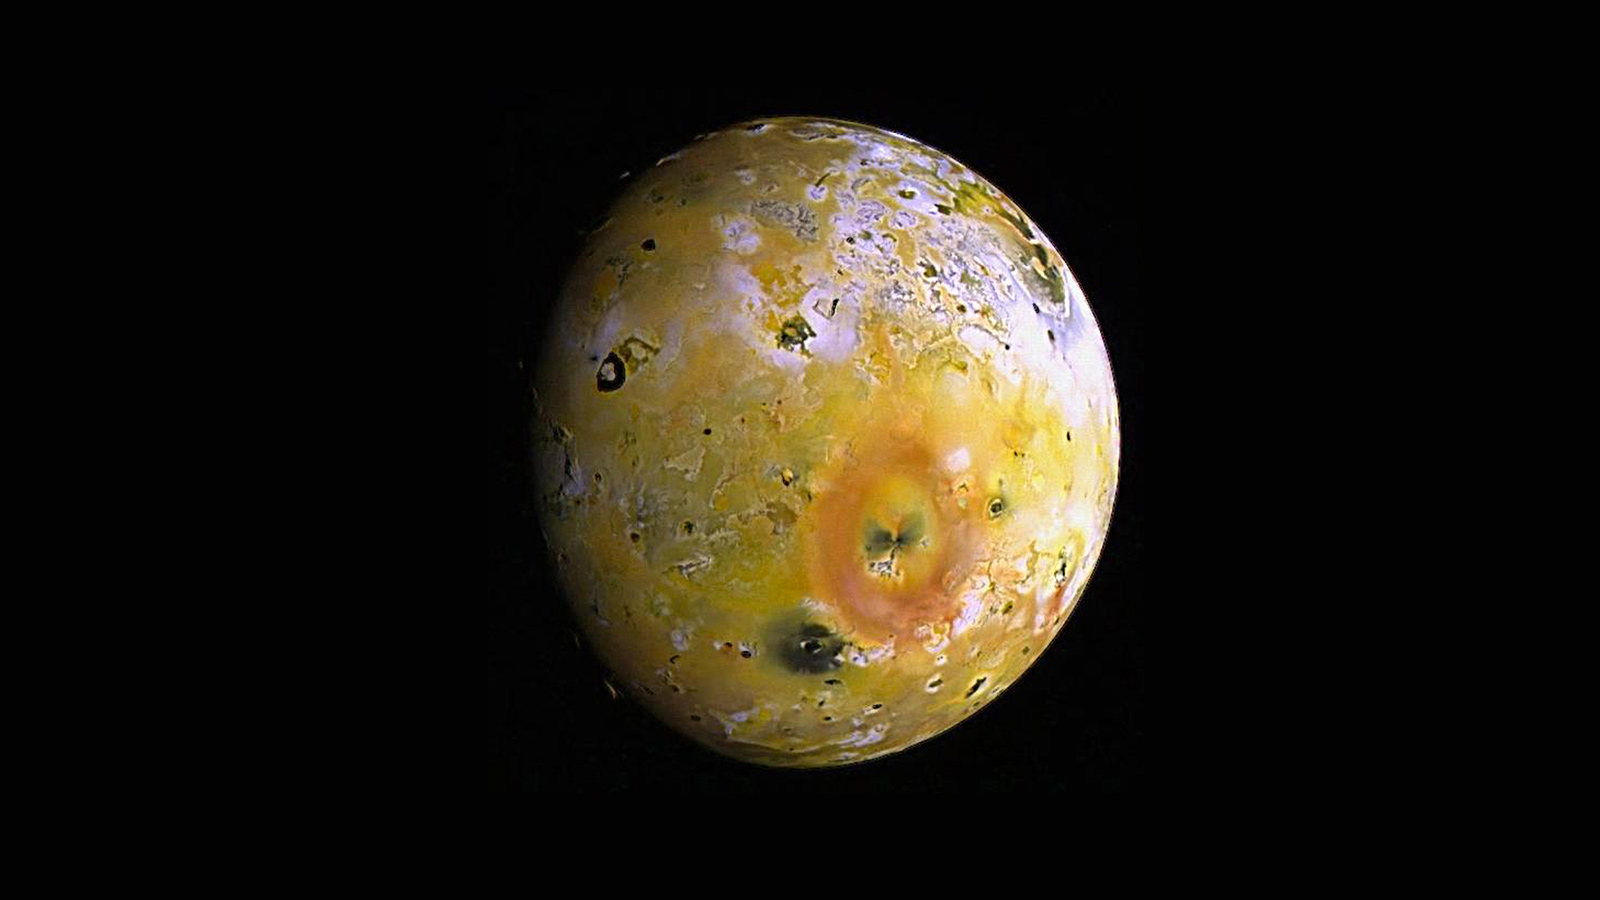
\includegraphics[width=0.6\textwidth]{img/giant-volcano-on-io-volcanic-moon-of-jupiter-expected-to-erupt.jpg}
    \caption{Io, luna de Júpiter seguiré escribiendo muchas cosas acá a ver qué pasa cuando me paso de la imagen. Debería ciertamente agregar variedad de palabrerío bastante extendido de manera que estafiguramuestremipunto}
    \label{fig:my_label}
\end{figure}

\lipsum[7]

\subsection{Y another}

\lipsum[8]